% 通途 fixture 论文（自造，原创占位内容，非真实论文）：单栏 article + 多文件源码树。
% 侧重覆盖点：flatten（\input 展开）、前导区 \title 槽位、\newtheorem/\newenvironment
% 声明驱动的环境分类、caption 可选参数、verbatim 与 lstlisting、bibtex 数据库。
\documentclass[11pt,a4paper]{article}

\usepackage{amsmath}
\usepackage{amssymb}
\usepackage{amsthm}
\usepackage{graphicx}
\usepackage{listings}

% 自定义命令与自定义环境。经 \input 进前导区——flatten 展开后 mask 才看得到这些声明，
% 因而 placeholderthm 判为 newtheorem-散文、takeaway 判为 newenvironment-散文。
\newcommand{\Pop}{\mathcal{P}}
\newcommand{\iter}[1]{x^{(#1)}}
\newcommand{\tol}{\varepsilon}
\newcommand{\Real}{\mathbb{R}}
\newcommand{\norm}[1]{\left\lVert #1 \right\rVert}
\newcommand{\fixturename}{placeholder iteration}

\theoremstyle{plain}
\newtheorem{placeholderthm}{Theorem}[section]
\newtheorem{placeholderlem}[placeholderthm]{Lemma}
\theoremstyle{definition}
\newtheorem{placeholderdef}{Definition}[section]

% 只给散文加装饰的自定义环境：mask 读 \newenvironment 的 begin 代码，没有委托任何
% 重环境，故判为散文——包裹留在掩码流里，内容照常翻译。
\newenvironment{takeaway}
  {\par\medskip\noindent\textbf{Takeaway.}\ \ignorespaces}
  {\par\medskip}


\title{On the Convergence of Placeholder Iterations}
\author{R. Placeholder\thanks{Fixture Institute for Synthetic Papers.}
  \and Q. Stand-In}
\date{}

\begin{document}
\maketitle

\begin{abstract}
We study a family of iterations built from an operator whose only defining
property is that it exists.  Under a contraction assumption that we simply
postulate, the iterates converge at a geometric rate, and the rate constant is
whatever the assumption says it is.  We restate this fact three times, tabulate
parameters that no experiment produced, and relegate the indices to an
appendix.  The paper is a test fixture: every number, citation and figure in it
was manufactured for the purpose of exercising a translation pipeline.
\end{abstract}

\section{Introduction}
\label{sec:intro}

Placeholder iterations arise whenever a system is described by a map that is
cheap to evaluate and inconvenient to invert.  This note collects the
elementary facts we rely on later.  Nothing here is new, and nothing here is
real: the document is a fixture, and its only job is to be translated.

We write $\iter{k}$ for the $k$-th iterate of the placeholder operator $\Pop$
acting on $\Real^{n}$, and we measure progress by the increment
$\norm{\iter{k+1} - \iter{k}}$.  The tolerance $\tol > 0$ is fixed throughout,
and the reader may assume it is small.  Roughly $70\%$ of the statements below
are immediate; the rest follow from Lemma~\ref{lem:contraction} together with
the estimates of \cite{fixture2021}.
% 一整段被注释掉的旧引言：连续整行注释会被 mask 合并成一个块，
% 往返自检要求它逐字节复原。
% \emph{Deleted:} an earlier version claimed a sharper rate; it did not survive
% contact with the counterexample in Appendix~\ref{app:details}.
Our contributions are deliberately mundane:

\begin{itemize}
  \item a restatement of the contraction estimate in the notation of
        Section~\ref{sec:method};
  \item a table of parameters that no experiment produced;
  \item an appendix that repeats the argument with more indices than are
        strictly necessary.
\end{itemize}

The remainder is organised as follows.\footnote{Sections are numbered in the
usual way and the appendix is lettered; we mention this only because a
footnote had to appear somewhere.}  Section~\ref{sec:method} fixes notation and
proves the one lemma we need, Section~\ref{sec:results} reports numbers that
were chosen rather than measured, and Appendix~\ref{app:details} expands the
recursion by hand.

\begin{takeaway}
Everything in this fixture is synthetic.  The numbers, the references and the
figures were generated for testing, and no claim in this document should be
believed by anyone, including its authors.
\end{takeaway}

\section{Setup and Notation}
\label{sec:method}

\subsection{The placeholder operator}
\label{sec:operator}

Let $\Pop \colon \Real^{n} \to \Real^{n}$ be a map, and let $\lambda \in [0,1)$
be a constant that we assume into existence.  We call the pair $(\Pop,\lambda)$
a \emph{\fixturename} whenever the following holds.

\begin{placeholderdef}
\label{def:stable}
The map $\Pop$ is \emph{placeholder-stable} with constant $\lambda$ if
$\norm{\Pop(y) - \Pop(z)} \le \lambda \norm{y - z}$ for all
$y, z \in \Real^{n}$.
\end{placeholderdef}

The iteration itself is the obvious one: starting from an arbitrary
$\iter{0} \in \Real^{n}$, set

\begin{equation}
  \label{eq:iteration}
  \iter{k+1} = \Pop\bigl(\iter{k}\bigr),
  \qquad k = 0, 1, 2, \dots
\end{equation}

Nothing in \eqref{eq:iteration} depends on the dimension $n$, which is why we
mention $n$ so often.

\begin{placeholderlem}
\label{lem:contraction}
If $(\Pop,\lambda)$ is a \fixturename{} with $\lambda < 1$, then the increments
of \eqref{eq:iteration} satisfy
$\norm{\iter{k+1} - \iter{k}} \le \lambda^{k}\norm{\iter{1} - \iter{0}}$ for
every $k \ge 0$.
\end{placeholderlem}

\begin{proof}
Apply Definition~\ref{def:stable} to consecutive iterates and unroll:
\begin{align}
  \norm{\iter{k+1} - \iter{k}}
    &\le \lambda \norm{\iter{k} - \iter{k-1}} \label{eq:step} \\
    &\le \lambda^{2} \norm{\iter{k-1} - \iter{k-2}} \nonumber \\
    &\le \lambda^{k} \norm{\iter{1} - \iter{0}} . \nonumber
\end{align}
The induction hidden in the last line is the routine one, and it is written out
in Appendix~\ref{app:details} for readers who enjoy indices.
\end{proof}

\subsection{Implementation sketch}
\label{sec:impl}

The reference implementation is four lines long and does not deserve a figure,
so we give it twice: once as code and once as a diagram.

\begin{lstlisting}[basicstyle=\ttfamily\small]
def placeholder_iteration(step, x0, tol=1e-6, max_iter=100):
    x = x0
    for k in range(max_iter):    # 100% synthetic; & no I/O here
        nxt = step(x)
        if norm(nxt - x) < tol:
            return nxt, k
        x = nxt
    return x, max_iter
\end{lstlisting}

Figure~\ref{fig:pipeline} shows the same thing with boxes.

\begin{figure}[t]
  \centering
  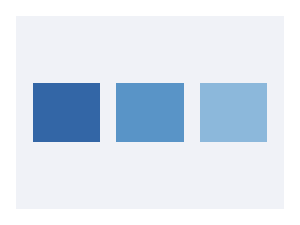
\includegraphics[width=0.55\linewidth]{figures/pipeline.pdf}
  \caption[Placeholder pipeline]{Schematic of the \fixturename: the leftmost
  block stands for whatever the reader has in mind, and the remaining blocks
  stand for it again.  About $30\%$ of the drawing is intentionally blank.}
  \label{fig:pipeline}
\end{figure}

\section{Results}
\label{sec:results}

\subsection{Parameters that were chosen, not measured}
\label{sec:params}

Table~\ref{tab:params} lists the settings used in the synthetic runs.  We stress
that no run took place; the table is here so that the pipeline has a
\texttt{tabular} to mask.

\begin{table}[t]
  \centering
  \caption[Synthetic parameters]{Parameters of the synthetic runs.  The last two
  columns report cost \& coverage for run \#3, and every entry was chosen to
  look plausible rather than to be true.}
  \label{tab:params}
  \begin{tabular}{lrr}
    \hline
    Stage     & Cost & Coverage \\
    \hline
    mask      & 0    & $100\%$   \\
    chunk     & 0    & $98\%$    \\
    translate & 12   & $95\%$    \\
    compile   & 3    & $99\%$    \\
    \hline
  \end{tabular}
\end{table}

\subsection{Ordered observations}
\label{sec:observations}

Reading Table~\ref{tab:params} in the light of Lemma~\ref{lem:contraction}, we
record the following, in order of decreasing confidence:

\begin{enumerate}
  \item the increments decrease geometrically, because we assumed they do;
  \item the constant $\lambda$ is smaller than one, by the same argument;
  \item the residual curve of Figure~\ref{fig:residuals} therefore slopes
        downwards, as drawn;
  \item any disagreement between items 1--3 and reality is a property of
        reality.
\end{enumerate}

\begin{figure}[b]
  \centering
  
\includegraphics[width=0.5\linewidth]{figures/residuals.png}
  \caption{Residual norms $\norm{\iter{k+1} - \iter{k}}$ against the iteration
  index $k$, drawn rather than computed.}
  \label{fig:residuals}
\end{figure}

\subsubsection{A remark on indices}
\label{sec:indices}

The index $k$ counts iterations and the index $i$ counts coordinates.  We have
seen manuscripts in which this convention is reversed \cite{stand2019}; we do
not recommend the practice, but we note it here so that a
\texttt{subsubsection} exists.


\section{Conclusion}
\label{sec:conclusion}

We have restated a contraction estimate in three notations and observed that
none of them changed the conclusion.  Future work will consist of restating it
in a fourth notation.  Readers looking for content are advised that this
document exists only so that a pipeline has something to translate.

\appendix
\section{Routine Computations}
\label{app:details}

\subsection{Expanding the recursion by hand}
\label{app:expand}

For completeness we unroll \eqref{eq:iteration} once more, this time writing
every index.  With $d_{k} = \norm{\iter{k+1} - \iter{k}}$ and $\lambda$ as in
Definition~\ref{def:stable},

\begin{equation}
  \label{eq:unrolled}
  d_{k} \le \lambda d_{k-1} \le \lambda^{2} d_{k-2} \le \cdots
        \le \lambda^{k} d_{0},
  \qquad k \ge 1 .
\end{equation}

Summing the geometric series gives
$\sum_{k \ge 0} d_{k} \le d_{0}/(1-\lambda)$, which is the bound quoted without
proof in \cite{placeholder2018}.

\begin{placeholderthm}
\label{thm:appendix}
Under the hypotheses of Lemma~\ref{lem:contraction} the sequence
$\{\iter{k}\}_{k \ge 0}$ is Cauchy, hence convergent, and its limit is a fixed
point of $\Pop$.
\end{placeholderthm}

\subsection{Command line used for the runs that did not happen}
\label{app:cli}

\begin{verbatim}
placeholder-run --iterations 100 --tolerance 1e-6 \
                --report out/report.json      # 100% reproducible
\end{verbatim}

The flag \texttt{-{}-report} writes a JSON summary; approximately $5\%$ of its
fields are ever read.


\bibliographystyle{plain}
\bibliography{refs}

\end{document}
